\documentclass[11pt,a4paper]{article}

% Packages
\usepackage{amsmath}
\usepackage{amssymb}
\usepackage{amsthm}
\usepackage[margin=1in]{geometry}
\usepackage{enumitem}
\usepackage{tikz}
\usepackage{pgfplots}
\usepackage{xcolor}
\pgfplotsset{compat=1.18}

% Custom commands
\newcommand{\stage}[1]{\textbf{\textcolor{blue}{#1}}}

% Title information
\title{Exercise Sheet 3: Bifurcations\\
Question 5 - Complete Solution}
\author{Methods of Applied Mathematics}
\date{}

\begin{document}

\maketitle

\section*{Problem Statement}

Show that a Hopf bifurcation happens in the system:
\begin{align*}
\frac{dx}{dt} &= 1 + x^2y - \mu x - x \\
\frac{dy}{dt} &= \mu x - x^2y
\end{align*}
as $\mu$ varies.

\vspace{10pt}
\hrule
\vspace{10pt}

\section{Step 1: Simplify and Understand System}

\subsection*{Rewrite first equation}

Collect terms in the first equation:
\[
\frac{dx}{dt} = 1 - x - \mu x + x^2y = 1 - (1+\mu)x + x^2y
\]

So the system is:
\begin{align*}
\dot{x} &= 1 - (1+\mu)x + x^2y \\
\dot{y} &= \mu x - x^2y
\end{align*}

\subsection*{Observe structure}

Notice that both equations involve the term $x^2y$ with opposite signs.

\subsection*{XYZ Analysis of System Structure}

\begin{itemize}[leftmargin=*]
\item \stage{STAGE X (What we have):} A coupled nonlinear system where both variables appear in both equations. The term $x^2y$ appears with opposite signs in the two equations, suggesting a conservation-like structure.

\item \stage{STAGE Y (Why this matters):} The symmetry in how $x^2y$ appears (positive in $\dot{x}$, negative in $\dot{y}$) hints at an underlying structure. If we add the equations:
\[
\dot{x} + \dot{y} = 1 - x - \mu x + x^2y + \mu x - x^2y = 1 - x
\]
The $x^2y$ terms cancel and $\mu x$ terms cancel, leaving a simple relationship. This kind of structure often appears in chemical reaction models (like the Brusselator family) where $x^2y$ represents an autocatalytic reaction rate.

\item \stage{STAGE Z (What to expect):} For Hopf bifurcations, we need:
\begin{itemize}
\item An equilibrium that doesn't move much with parameter (or moves in a controlled way)
\item Eigenvalues that are complex for a range of $\mu$
\item Real part of eigenvalues crossing zero at critical $\mu$
\item Imaginary part remaining nonzero at crossing
\end{itemize}
The nonlinearity and coupling suggest oscillatory behavior is possible.
\end{itemize}

\vspace{10pt}
\hrule
\vspace{10pt}

\section{Step 2: Find Equilibria}

\subsection*{Set up equilibrium conditions}

For equilibria, we require $\dot{x} = 0$ and $\dot{y} = 0$:
\begin{align*}
1 - (1+\mu)x + x^2y &= 0 \quad \cdots (1)\\
\mu x - x^2y &= 0 \quad \cdots (2)
\end{align*}

\subsection*{Solve systematically}

From equation (2):
\[
x(\mu - xy) = 0
\]

This gives either $x = 0$ or $xy = \mu$.

\textbf{Case 1: $x = 0$}

Substitute into equation (1):
\[
1 - 0 + 0 = 1 = 0 \quad \text{Contradiction!}
\]

So $x = 0$ is not an equilibrium.

\textbf{Case 2: $xy = \mu$}

This means $y = \mu/x$ (assuming $x \neq 0$).

Substitute into equation (1):
\begin{align*}
1 - (1+\mu)x + x^2 \cdot \frac{\mu}{x} &= 0 \\
1 - (1+\mu)x + x\mu &= 0 \\
1 - x - \mu x + \mu x &= 0 \\
1 - x &= 0
\end{align*}

Therefore: $x = 1$

And: $y = \mu/1 = \mu$

\subsection*{Equilibrium}

\[
\boxed{(x^*, y^*) = (1, \mu)}
\]

\subsection*{Verify equilibrium}

Check equation (1): $1 - (1+\mu)(1) + (1)^2(\mu) = 1 - 1 - \mu + \mu = 0$ ✓

Check equation (2): $\mu(1) - (1)^2(\mu) = \mu - \mu = 0$ ✓

\subsection*{XYZ Analysis of Equilibrium}

\begin{itemize}[leftmargin=*]
\item \stage{STAGE X (What we found):} Unique equilibrium at $(1, \mu)$. The $x$-coordinate is constant ($x^* = 1$) while the $y$-coordinate moves linearly with parameter ($y^* = \mu$).

\item \stage{STAGE Y (Why this structure):} The equilibrium position in $y$ tracks the parameter $\mu$ directly. This is unusual but not unprecedented. The key observation is that from $\mu x = x^2 y$ at equilibrium, we have $y = \mu/x$. Since $x = 1$ was forced by the first equation (independent of $\mu$), we get $y = \mu$ automatically. The first equation $1 - x + x^2y - \mu x = 0$ becomes $1 - x = 0$ after using $x^2y = \mu x$ from the second equation, giving $x = 1$ regardless of $\mu$.

\item \stage{STAGE Z (What this means):} The equilibrium moves through the phase plane as $\mu$ varies, but only in the $y$-direction. For Hopf bifurcation, we need the stability at this moving equilibrium to change - specifically, eigenvalues must become complex with zero real part at some critical $\mu^*$. Let's compute the Jacobian to investigate stability.
\end{itemize}

\vspace{10pt}
\hrule
\vspace{10pt}

\section{Step 3: Compute Jacobian Matrix}

\subsection*{Partial derivatives}

For $f(x,y) = 1 - (1+\mu)x + x^2y$ and $g(x,y) = \mu x - x^2y$:

\begin{align*}
\frac{\partial f}{\partial x} &= -(1+\mu) + 2xy \\
\frac{\partial f}{\partial y} &= x^2 \\
\frac{\partial g}{\partial x} &= \mu - 2xy \\
\frac{\partial g}{\partial y} &= -x^2
\end{align*}

\subsection*{Jacobian at general point}

\[
J(x,y) = \begin{pmatrix}
-(1+\mu) + 2xy & x^2 \\
\mu - 2xy & -x^2
\end{pmatrix}
\]

\subsection*{Jacobian at equilibrium $(1, \mu)$}

Substitute $x = 1, y = \mu$:

\begin{align*}
\frac{\partial f}{\partial x}\bigg|_{(1,\mu)} &= -(1+\mu) + 2(1)(\mu) = -1 - \mu + 2\mu = \mu - 1 \\
\frac{\partial f}{\partial y}\bigg|_{(1,\mu)} &= (1)^2 = 1 \\
\frac{\partial g}{\partial x}\bigg|_{(1,\mu)} &= \mu - 2(1)(\mu) = \mu - 2\mu = -\mu \\
\frac{\partial g}{\partial y}\bigg|_{(1,\mu)} &= -(1)^2 = -1
\end{align*}

Therefore:
\[
J(1,\mu) = \begin{pmatrix}
\mu - 1 & 1 \\
-\mu & -1
\end{pmatrix}
\]

\subsection*{XYZ Analysis of Jacobian}

\begin{itemize}[leftmargin=*]
\item \stage{STAGE X (What we have):} A parameter-dependent Jacobian with all four entries depending on $\mu$. Unlike previous examples with diagonal or simple structure, this is a fully-populated 2×2 matrix.

\item \stage{STAGE Y (Why this structure):} The Jacobian entries show how the linearized dynamics depend on $\mu$:
\begin{itemize}
\item Upper-left $(\mu - 1)$: Self-feedback in $x$-equation, changes sign at $\mu = 1$
\item Upper-right $(1)$: Constant positive coupling from $y$ to $\dot{x}$
\item Lower-left $(-\mu)$: Negative feedback from $x$ to $\dot{y}$, grows with $\mu$
\item Lower-right $(-1)$: Constant negative self-feedback in $y$-equation (damping)
\end{itemize}
The non-diagonal structure means the eigenvalues will generally be complex. The parameter-dependence in multiple entries suggests eigenvalues will move in the complex plane as $\mu$ varies.

\item \stage{STAGE Z (What to compute):} To identify a Hopf bifurcation, we need:
\begin{enumerate}
\item Find the eigenvalues as functions of $\mu$
\item Identify critical value $\mu^*$ where real part is zero
\item Verify imaginary part is nonzero at $\mu^*$
\item Check that real part crosses zero transversely (nonzero derivative)
\end{enumerate}
Let's compute the characteristic equation.
\end{itemize}

\vspace{10pt}
\hrule
\vspace{10pt}

\section{Step 4: Find Eigenvalues}

\subsection*{Compute trace and determinant}

\begin{align*}
\text{Trace: } \tau &= (\mu - 1) + (-1) = \mu - 2 \\
\text{Determinant: } \Delta &= (\mu - 1)(-1) - (1)(-\mu) \\
&= -\mu + 1 + \mu = 1
\end{align*}

Notice: $\Delta = 1 > 0$ for all $\mu$ (constant!)

\subsection*{Characteristic equation}

\[
\lambda^2 - \tau\lambda + \Delta = 0
\]
\[
\lambda^2 - (\mu - 2)\lambda + 1 = 0
\]

\subsection*{Solve for eigenvalues}

Using quadratic formula:
\[
\lambda = \frac{(\mu - 2) \pm \sqrt{(\mu-2)^2 - 4}}{2}
\]

\subsection*{Analyze discriminant}

Let $\Delta_{disc} = (\mu-2)^2 - 4$

\begin{align*}
\Delta_{disc} > 0 &\quad \Rightarrow \quad \text{real eigenvalues} \\
\Delta_{disc} = 0 &\quad \Rightarrow \quad \text{repeated real eigenvalue} \\
\Delta_{disc} < 0 &\quad \Rightarrow \quad \text{complex eigenvalues}
\end{align*}

$(\mu-2)^2 - 4 = 0$ when $|\mu - 2| = 2$, i.e., $\mu = 0$ or $\mu = 4$

\begin{itemize}
\item For $\mu < 0$: $\Delta_{disc} > 0$ (real eigenvalues)
\item For $0 < \mu < 4$: $\Delta_{disc} < 0$ (complex eigenvalues)
\item For $\mu > 4$: $\Delta_{disc} > 0$ (real eigenvalues)
\end{itemize}

\subsection*{Complex eigenvalues for $0 < \mu < 4$}

When eigenvalues are complex:
\[
\lambda = \frac{\mu - 2}{2} \pm i\frac{\sqrt{4 - (\mu-2)^2}}{2}
\]

Define:
\begin{align*}
\rho(\mu) &= \text{Re}(\lambda) = \frac{\mu - 2}{2} \\
\omega(\mu) &= \text{Im}(\lambda) = \pm\frac{\sqrt{4 - (\mu-2)^2}}{2}
\end{align*}

\subsection*{XYZ Analysis of Eigenvalue Structure}

\begin{itemize}[leftmargin=*]
\item \stage{STAGE X (What we found):} The determinant is constant ($\Delta = 1$) but the trace varies linearly with $\mu$ ($\tau = \mu - 2$). For $0 < \mu < 4$, eigenvalues are complex conjugates.

\item \stage{STAGE Y (Why complex eigenvalues):} The constant positive determinant $\Delta = 1$ ensures:
\[
\lambda_1 \cdot \lambda_2 = 1 > 0
\]
So eigenvalues have the same sign (both positive, both negative, or complex conjugates). The discriminant:
\[
\tau^2 - 4\Delta = (\mu-2)^2 - 4
\]
is negative when $|\mu - 2| < 2$, forcing eigenvalues to be complex in this range. The geometry: in the trace-determinant plane, the point $(\tau, \Delta) = (\mu-2, 1)$ moves horizontally (at fixed $\Delta = 1$) as $\mu$ varies. It crosses into the "complex eigenvalue" region when $|\tau| < 2\sqrt{\Delta} = 2$.

\item \stage{STAGE Z (What this means):} Complex eigenvalues indicate oscillatory behavior (spirals in phase plane). The real part $\rho(\mu) = (\mu-2)/2$ determines whether spirals approach equilibrium (stable, $\rho < 0$) or recede (unstable, $\rho > 0$). The critical value $\rho = 0$ occurs at $\mu = 2$. This is where the Hopf bifurcation happens!
\end{itemize}

\vspace{10pt}
\hrule
\vspace{10pt}

\section{Step 5: Identify Hopf Bifurcation Point}

\subsection*{Find critical parameter value}

Real part is zero when:
\[
\rho(\mu) = \frac{\mu - 2}{2} = 0 \quad \Rightarrow \quad \boxed{\mu^* = 2}
\]

\subsection*{Check imaginary part at critical value}

At $\mu = 2$:
\[
\omega(2) = \pm\frac{\sqrt{4 - (2-2)^2}}{2} = \pm\frac{\sqrt{4}}{2} = \pm 1
\]

So the eigenvalues at $\mu = 2$ are:
\[
\lambda = 0 \pm i(1) = \pm i
\]

Verification by substituting into characteristic equation:
\[
\lambda^2 - (2-2)\lambda + 1 = \lambda^2 + 1 = 0 \quad \Rightarrow \quad \lambda = \pm i \quad \checkmark
\]

\subsection*{Verify imaginary part is nonzero}

\[
\omega(2) = 1 \neq 0 \quad \checkmark
\]

\subsection*{XYZ Analysis of Critical Point}

\begin{itemize}[leftmargin=*]
\item \stage{STAGE X (What we found):} At $\mu = 2$, the equilibrium $(1, 2)$ has purely imaginary eigenvalues $\lambda = \pm i$.

\item \stage{STAGE Y (Why this is special):} Purely imaginary eigenvalues mean the linearized system near the equilibrium has periodic solutions - closed orbits with frequency $\omega = 1$ (period $2\pi$). The zero real part means these orbits neither grow nor decay - they're neutral. This is the borderline between:
\begin{itemize}
\item $\mu < 2$: $\rho < 0$, stable spiral (trajectories approach equilibrium)
\item $\mu = 2$: $\rho = 0$, center-like behavior in linearization
\item $\mu > 2$: $\rho > 0$, unstable spiral (trajectories recede from equilibrium)
\end{itemize}
At exactly $\mu = 2$, we're at a critical transition point.

\item \stage{STAGE Z (What happens):} This is a necessary condition for Hopf bifurcation, but not sufficient. We still need to verify that:
\begin{enumerate}
\item The real part crosses zero transversely (derivative nonzero)
\item The system is "generic" (non-degenerate)
\end{enumerate}
The full Hopf bifurcation theorem tells us that under these conditions, a limit cycle (periodic orbit) emerges for $\mu$ near 2. Let's verify the transversality condition.
\end{itemize}

\vspace{10pt}
\hrule
\vspace{10pt}

\section{Step 6: Verify Hopf Bifurcation Conditions}

\subsection*{Condition (B1): Equilibrium exists}

At $\mu = 2$, the equilibrium is $(1, 2)$. ✓

\subsection*{Condition (B2): Eigenvalues purely imaginary}

At $\mu = 2$: $\lambda = \pm i$ (pure imaginary). ✓

\subsection*{Condition (G1): Imaginary part nonzero}

\[
\omega(2) = 1 \neq 0 \quad \checkmark
\]

\subsection*{Condition (G2): Real part crosses zero transversely}

Compute the derivative of the real part with respect to $\mu$:
\[
\frac{d\rho}{d\mu} = \frac{d}{d\mu}\left[\frac{\mu - 2}{2}\right] = \frac{1}{2}
\]

At $\mu = 2$:
\[
\frac{d\rho}{d\mu}\bigg|_{\mu=2} = \frac{1}{2} \neq 0 \quad \checkmark
\]

Since the derivative is positive, the real part crosses from negative to positive as $\mu$ increases through 2.

\subsection*{Conclusion}

All Hopf bifurcation conditions are satisfied:

\[
\boxed{\text{HOPF BIFURCATION at } \mu = 2, \text{ equilibrium } (1, 2)}
\]

\subsection*{XYZ Analysis of Verification}

\begin{itemize}[leftmargin=*]
\item \stage{STAGE X (What we verified):} All four conditions (B1, B2, G1, G2) for a Hopf bifurcation hold at $\mu = 2$.

\item \stage{STAGE Y (Why each condition matters):}
\begin{itemize}
\item \textbf{(B1) Equilibrium exists}: Fundamental - need a reference point for bifurcation
\item \textbf{(B2) Pure imaginary eigenvalues}: Indicates neutrally stable oscillations in linearization at critical point
\item \textbf{(G1) Imaginary part nonzero}: Ensures genuine oscillation (frequency $\omega = 1$, not degenerate case $\omega = 0$). Guarantees the periodic behavior is robust
\item \textbf{(G2) Transverse crossing}: Ensures the stability change is non-degenerate. The derivative $d\rho/d\mu = 1/2 > 0$ means:
  \begin{itemize}
  \item For $\mu$ slightly less than 2: $\rho < 0$ (stable spiral)
  \item For $\mu$ slightly greater than 2: $\rho > 0$ (unstable spiral)
  \end{itemize}
  The crossing is transverse (not tangential), guaranteeing a limit cycle emerges rather than higher-order degeneracy
\end{itemize}

\item \stage{STAGE Z (What this guarantees):} By the Hopf Bifurcation Theorem (Section 14 of lecture notes, pages 53-55), the system exhibits:
\begin{itemize}
\item For $\mu < 2$: Stable equilibrium at $(1, \mu)$, no periodic orbits nearby
\item For $\mu$ near 2: A periodic orbit (limit cycle) emerges
\item The amplitude of the limit cycle grows like $\sqrt{|\mu - 2|}$ near the bifurcation
\item Whether the bifurcation is supercritical (stable limit cycle for $\mu > 2$) or subcritical (unstable limit cycle for $\mu < 2$) depends on the sign of the first Lyapunov coefficient $\ell_1$ (not computed here)
\end{itemize}
\end{itemize}

\vspace{10pt}
\hrule
\vspace{10pt}

\section{Step 7: Characterize the Bifurcation}

\subsection*{Eigenvalue paths in complex plane}

As $\mu$ varies, the eigenvalues trace paths:

\textbf{For $0 < \mu < 4$ (complex eigenvalues):}
\[
\lambda(\mu) = \frac{\mu - 2}{2} \pm i\frac{\sqrt{4 - (\mu-2)^2}}{2}
\]

Key values:
\begin{align*}
\mu = 0: \quad & \lambda = -1 \pm i \cdot 0 = -1 \quad \text{(repeated)} \\
\mu = 1: \quad & \lambda = -\frac{1}{2} \pm i\frac{\sqrt{3}}{2} \\
\mu = 2: \quad & \lambda = 0 \pm i \\
\mu = 3: \quad & \lambda = +\frac{1}{2} \pm i\frac{\sqrt{3}}{2} \\
\mu = 4: \quad & \lambda = +1 \pm i \cdot 0 = +1 \quad \text{(repeated)}
\end{align*}

\subsection*{Eigenvalue trajectory}

\begin{center}
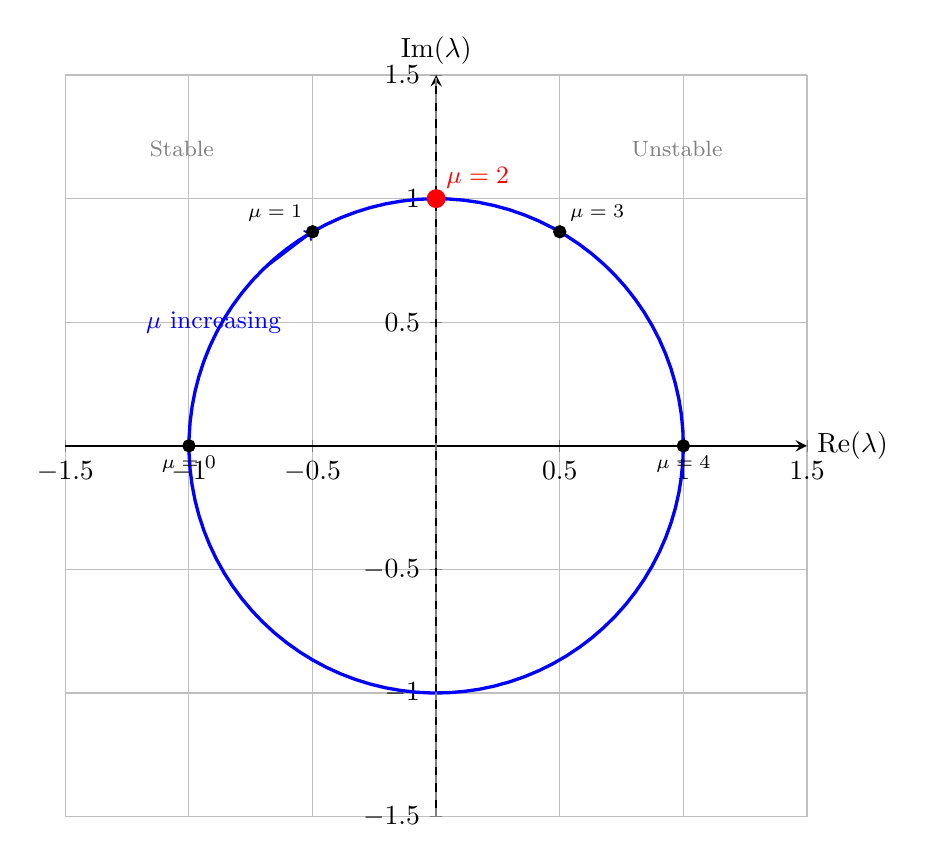
\begin{tikzpicture}
\begin{axis}[
    width=11cm,
    height=11cm,
    xlabel={$\text{Re}(\lambda)$},
    ylabel={$\text{Im}(\lambda)$},
    xmin=-1.5, xmax=1.5,
    ymin=-1.5, ymax=1.5,
    grid=major,
    axis lines=middle,
    thick,
    axis equal,
    every axis x label/.style={at={(current axis.right of origin)},anchor=west},
    every axis y label/.style={at={(current axis.above origin)},anchor=south}
]

% Circle representing eigenvalue path
\addplot[blue, very thick, domain=0:360, samples=100] ({cos(x)}, {sin(x)});

% Mark special points
\addplot[mark=*, mark size=3pt, red, only marks] coordinates {(0, 1)};
\node[red, above right, font=\small] at (axis cs:0,1) {$\mu = 2$};

\addplot[mark=*, mark size=2pt, black, only marks] coordinates {(-1, 0)};
\node[below, font=\scriptsize] at (axis cs:-1,0) {$\mu=0$};

\addplot[mark=*, mark size=2pt, black, only marks] coordinates {(1, 0)};
\node[below, font=\scriptsize] at (axis cs:1,0) {$\mu=4$};

\addplot[mark=*, mark size=2pt, black, only marks] coordinates {(-0.5, 0.866)};
\node[above left, font=\scriptsize] at (axis cs:-0.5,0.866) {$\mu=1$};

\addplot[mark=*, mark size=2pt, black, only marks] coordinates {(0.5, 0.866)};
\node[above right, font=\scriptsize] at (axis cs:0.5,0.866) {$\mu=3$};

% Arrow showing direction
\draw[->, thick, blue] (axis cs:-0.7,0.714) -- (axis cs:-0.5,0.866);
\node[blue, font=\small] at (axis cs:-0.9,0.5) {$\mu$ increasing};

% Stable/Unstable regions
\draw[dashed, gray] (axis cs:0,-1.5) -- (axis cs:0,1.5);
\node[gray, font=\footnotesize, anchor=west] at (axis cs:-1.2,1.2) {Stable};
\node[gray, font=\footnotesize, anchor=east] at (axis cs:1.2,1.2) {Unstable};

\end{axis}
\end{tikzpicture}
\end{center}

\subsection*{Stability summary}

\begin{center}
\begin{tabular}{|c|c|c|}
\hline
\textbf{Parameter Range} & \textbf{Eigenvalues} & \textbf{Stability} \\
\hline
$\mu < 2$ & $\text{Re}(\lambda) < 0$ & Stable spiral \\
\hline
$\mu = 2$ & $\lambda = \pm i$ & Neutral (Hopf point) \\
\hline
$\mu > 2$ & $\text{Re}(\lambda) > 0$ & Unstable spiral \\
\hline
\end{tabular}
\end{center}

\subsection*{XYZ Analysis of Eigenvalue Evolution}

\begin{itemize}[leftmargin=*]
\item \stage{STAGE X (What we see):} Eigenvalues move counterclockwise around a circle of radius 1 in the complex plane as $\mu$ increases from 0 to 4. They cross the imaginary axis (Hopf bifurcation) at $\mu = 2$.

\item \stage{STAGE Y (Why circular path):} The constant determinant $\Delta = 1$ means:
\[
|\lambda_1| \cdot |\lambda_2| = 1
\]
For complex conjugate eigenvalues: $\lambda = \rho \pm i\omega$, we have $|\lambda|^2 = \rho^2 + \omega^2$.
So: $|\lambda|^2 = \Delta = 1$, meaning eigenvalues lie on the unit circle in the complex plane.

As $\mu$ varies from 0 to 4, the trace $\tau = \mu - 2$ varies from $-2$ to $+2$. The eigenvalue formula:
\[
\lambda = \frac{\tau}{2} \pm i\frac{\sqrt{4\Delta - \tau^2}}{2} = \frac{\tau}{2} \pm i\frac{\sqrt{4 - \tau^2}}{2}
\]
with $\Delta = 1$ gives a parametric equation for a semicircle. Setting $\tau = 2\cos\theta$ (varies from $-2$ to $+2$ as $\theta$ goes from $\pi$ to $0$), we get:
\[
\lambda = \cos\theta \pm i\sin\theta = e^{\pm i\theta}
\]
This is precisely the unit circle! The angle $\theta$ relates to $\mu$ by $\cos\theta = (\mu-2)/2$.

\item \stage{STAGE Z (What this means physically):} The circular trajectory is special to this system. As $\mu$ increases:
\begin{itemize}
\item Eigenvalues start at $\lambda = -1$ (repeated, $\mu = 0$)
\item Split into complex conjugates and move through left half-plane (stable spirals)
\item Cross imaginary axis at $\mu = 2$ (Hopf bifurcation) with frequency $\omega = 1$
\item Continue into right half-plane (unstable spirals)
\item Reconverge to $\lambda = +1$ (repeated, $\mu = 4$)
\end{itemize}
The Hopf bifurcation occurs exactly when the circular path crosses the imaginary axis. The frequency of emerging oscillations matches the imaginary part at crossing: $\omega(2) = 1$, giving period $T = 2\pi/\omega = 2\pi$.
\end{itemize}

\vspace{10pt}
\hrule
\vspace{10pt}

\section{Step 8: Physical Interpretation}

\subsection*{System behavior across bifurcation}

\textbf{For $\mu < 2$:}
\begin{itemize}
\item Equilibrium $(1, \mu)$ is stable spiral
\item Trajectories spiral inward toward equilibrium
\item System reaches steady state (no oscillations in long term)
\end{itemize}

\textbf{At $\mu = 2$:}
\begin{itemize}
\item Equilibrium $(1, 2)$ has purely imaginary eigenvalues
\item Linearization shows neutral cycles (neither growing nor decaying)
\item Critical transition point
\end{itemize}

\textbf{For $\mu > 2$ (just above bifurcation):}
\begin{itemize}
\item Equilibrium $(1, \mu)$ is unstable spiral
\item A limit cycle emerges (periodic orbit)
\item System exhibits sustained oscillations
\end{itemize}

\subsection*{Expected dynamics near bifurcation}

If supercritical (most common):
\begin{itemize}
\item For $\mu \lesssim 2$: Stable equilibrium, small perturbations decay
\item For $\mu \gtrsim 2$: Small stable limit cycle emerges, radius $\propto \sqrt{\mu - 2}$
\item Trajectories approach limit cycle from inside and outside
\end{itemize}

If subcritical (less common):
\begin{itemize}
\item For $\mu \lesssim 2$: Small unstable limit cycle exists below bifurcation
\item For $\mu \gtrsim 2$: Equilibrium unstable, trajectories diverge or approach distant attractor
\end{itemize}

\subsection*{XYZ Analysis of Physical Behavior}

\begin{itemize}[leftmargin=*]
\item \stage{STAGE X (What happens):} The system transitions from steady state to oscillatory behavior as $\mu$ crosses 2. Sustained periodic oscillations emerge where there were none before.

\item \stage{STAGE Y (Why oscillations emerge):} Near the Hopf bifurcation, the linearized dynamics exhibit rotation (from imaginary part of eigenvalues) and growth/decay (from real part). When real part is negative ($\mu < 2$), the rotation is damped and trajectories spiral inward. When real part becomes positive ($\mu > 2$), the rotation is amplified and trajectories spiral outward from equilibrium.

But the system is nonlinear - the terms $x^2y$ and $-x^2y$ provide nonlinear feedback. As amplitude grows beyond equilibrium, these nonlinear terms eventually balance the linear instability, stabilizing the trajectory into a limit cycle. The Hopf Bifurcation Theorem guarantees this balance creates a periodic orbit for $\mu$ near the critical value.

\item \stage{STAGE Z (What this represents):} Hopf bifurcations model the onset of oscillations in many physical systems:
\begin{itemize}
\item \textbf{Chemical reactions}: Oscillating concentrations (e.g., Belousov-Zhabotinsky reaction)
\item \textbf{Biological systems}: Circadian rhythms, neural firing patterns, population cycles
\item \textbf{Mechanical systems}: Flutter instability in aircraft wings
\item \textbf{Electrical circuits}: Oscillator circuits, laser dynamics
\item \textbf{Climate models}: Periodic climate patterns (e.g., El Niño)
\end{itemize}
The parameter $\mu$ represents a control parameter (temperature, reaction rate, feedback gain, etc.) that, when varied, causes the system to spontaneously begin oscillating. This is a qualitative change in dynamics - from equilibrium to periodic motion.
\end{itemize}

\vspace{10pt}
\hrule
\vspace{10pt}

\section{Summary}

\subsection*{System}

\begin{align*}
\dot{x} &= 1 - (1+\mu)x + x^2y \\
\dot{y} &= \mu x - x^2y
\end{align*}

\subsection*{Equilibrium}

\[
(x^*, y^*) = (1, \mu) \quad \text{for all } \mu
\]

\subsection*{Jacobian at equilibrium}

\[
J(1,\mu) = \begin{pmatrix}
\mu - 1 & 1 \\
-\mu & -1
\end{pmatrix}
\]

\subsection*{Eigenvalues}

\begin{align*}
\tau &= \mu - 2 \\
\Delta &= 1 \\
\lambda &= \frac{\mu - 2}{2} \pm i\frac{\sqrt{4 - (\mu-2)^2}}{2} \quad \text{for } 0 < \mu < 4
\end{align*}

\subsection*{Hopf Bifurcation}

\[
\boxed{\text{Occurs at } \mu^* = 2, \text{ equilibrium } (1, 2)}
\]

\textbf{Verification:}
\begin{itemize}
\item[(B1)] Equilibrium $(1, 2)$ exists ✓
\item[(B2)] Eigenvalues $\lambda = \pm i$ (purely imaginary) ✓
\item[(G1)] Frequency $\omega(2) = 1 \neq 0$ ✓
\item[(G2)] Transversality: $d\rho/d\mu = 1/2 \neq 0$ ✓
\end{itemize}

\textbf{Dynamics:}
\begin{itemize}
\item $\mu < 2$: Stable spiral → steady state
\item $\mu = 2$: Purely imaginary eigenvalues → Hopf bifurcation
\item $\mu > 2$: Unstable spiral → limit cycle emerges
\end{itemize}

\textbf{Key insight:} The constant determinant ($\Delta = 1$) constrains eigenvalues to unit circle in complex plane. As trace varies linearly with $\mu$, eigenvalues sweep around circle, crossing imaginary axis at $\mu = 2$ - the Hopf bifurcation point where oscillatory behavior emerges.

\end{document}
